\documentclass[11pt,a4paper]{article}
\usepackage[T1]{fontenc}
\usepackage[utf8]{inputenc}
\usepackage{lmodern}
\usepackage[margin=2.3cm]{geometry}
\usepackage{amsmath,amssymb}
\usepackage{booktabs}
\usepackage{graphicx}
\usepackage{caption}
\usepackage{float}
\usepackage{microtype}
\usepackage{xcolor}
\usepackage{enumitem}
\usepackage[colorlinks=true,linkcolor=blue!50!black,citecolor=blue!50!black,urlcolor=blue!50!black]{hyperref}
\setlist{itemsep=2pt,topsep=4pt}
\captionsetup{font=small,labelfont=bf}
\newcommand{\best}[1]{\textbf{#1}}

\title{\textbf{Benchmarking FSRS against a\\Continuous-Time Bayesian Retention Model\\on Anki Review Logs}\\[4pt]
\large Evaluation protocol, implementation and results}
\author{Final Year Project --- Axiom (\texttt{BayesianScheduler} branch)}
\date{October 2026}

\begin{document}
\maketitle

\begin{abstract}
\noindent We build a reproducible, leakage-free evaluation pipeline that compares the Free Spaced Repetition Scheduler (FSRS-6) with our continuous-time Bayesian dynamic retention model (DLM) and with Half-Life Regression (HLR, Settles \& Meeder 2016). All models are scored on exactly the same 95{,}400 held-out review events from 100 users of the public \texttt{anki-revlogs-10k} dataset, using a per-user time split and strictly one-step-ahead prediction. Each card's memory state is reconstructed by replaying its review history in chronological order. On log loss, Brier score, AUC and calibration (ECE), FSRS-6 with per-user optimised parameters is the best model overall (log loss 0.379, AUC 0.777, ECE 0.009) and in every review-gap bin. Our model (log loss 0.422, AUC 0.692, ECE 0.025) is significantly worse than both FSRS-6 variants under a user-clustered paired bootstrap, but far better than HLR (log loss 0.680, AUC 0.555). Adding the practice-dependent decay term $\kappa$ changes nothing measurable. The Gibbs sampler did not converge at 2{,}000 iterations ($\hat R_\lambda \approx 2.4$), so the results for our model are provisional. We give evidence that its predictions are nonetheless insensitive to the poorly mixed parameters.
\end{abstract}

\section{Introduction}
Spaced repetition systems schedule reviews from a predicted probability of recall. Our project proposes a continuous-time Bayesian dynamic linear model (DLM) of human retention, in which a latent memory state decays between reviews and is updated by each outcome. Earlier project updates compared the DLM with static baselines: a lagged logistic regression and HLR. This report adds the comparison that a reviewer will expect first: FSRS, the open-source scheduler used by Anki and the strongest widely used public baseline.

The task was to:
\begin{enumerate}
  \item implement a working evaluation pipeline for FSRS on the \texttt{anki-revlogs-10k} dataset (Open Spaced Repetition);
  \item reconstruct each card's memory state by replaying its review history chronologically with the official FSRS implementation;
  \item predict recall probabilities for held-out reviews without data leakage;
  \item compare FSRS with our model on exactly the same test events, using log loss, Brier score, AUC and calibration metrics;
  \item document the protocol, implementation choices and results, with reproducible code.
\end{enumerate}
HLR, the model of the Duolingo paper, is included as a third reference point.

\section{Data}
\paragraph{Source.} \texttt{anki-revlogs-10k} is a gated Hugging Face dataset with one review log per Anki user. Each row is one review, with the card id, the day offset, the rating (1 = Again, 2 = Hard, 3 = Good, 4 = Easy), the card state and the elapsed time. We sample 100 users with a fixed seed (0), and at most 1{,}000 cards per user, sampled with the same seed. The cap keeps the Gibbs sampler tractable. A 5-user pilot showed that 1{,}000 cards per user, unlike 300, leaves almost every user with enough data for the FSRS optimiser.

\paragraph{Event definition.}
\begin{itemize}
  \item Rows with rating 0 (manual reschedules) are dropped.
  \item Filtered-deck reviews (state 4) are \emph{kept}. They carry real ratings and durations, and dropping them gave FSRS wrong gaps (in one case 515 days instead of 1).
  \item Cards whose first kept review is not a new-card review are dropped, because their history is truncated and their memory state cannot be rebuilt.
  \item The label is $y=1$ (recalled) if the rating is above 1.
  \item Review gaps are recomputed over the kept rows, so every model sees identical gaps.
\end{itemize}

\begin{table}[H]
\centering
\caption{The full run (\texttt{results/full\_u100\_c1000}).}
\label{tab:data}
\begin{tabular}{lr@{\hspace{2.5em}}lr}
\toprule
Users & 100 & Train events & 606{,}364 \\
Cards & 99{,}074 & Test events & 162{,}294 \\
Review events & 768{,}658 & Scored test events & 95{,}400 \\
 & & Recall rate (scored) & 0.831 \\
\bottomrule
\end{tabular}
\end{table}

\section{Evaluation protocol}
\paragraph{Split.} For each user, the cutoff is the 80th percentile of that user's review days. Reviews before the cutoff are \textsc{train}, and the rest are \textsc{test}. All model parameters are fitted on \textsc{train} rows only and frozen during the test period.

\paragraph{Scored events.} A \textsc{test} review is scored if it is not the card's first review and its gap is at least one day. This is the srs-benchmark convention of scoring inter-day reviews. Same-day and first reviews are still fed to the models as history, but are never scored.

\paragraph{One-step-ahead prediction.} To predict scored event $k$, a model may use the card's entire history before $k$, including earlier test reviews and their outcomes. It may not use event $k$ or anything after it. This mirrors how a scheduler is used in practice.

\paragraph{Leakage tests.} The pipeline has 260 automated tests. Those that enforce the protocol check that:
\begin{itemize}
  \item no \textsc{train} event lies at or after a user's cutoff;
  \item changing a scored event's own outcome, or any later outcome, never changes its prediction (checked for every model);
  \item flipping every \textsc{test} label leaves all five models' predictions identical;
  \item users and cards seen only in \textsc{test} use our model's cold-start path;
  \item all five models predict exactly the same set of event ids.
\end{itemize}

\section{Models}
\paragraph{FSRS-6 (default and optimised).} We use the official \texttt{py-fsrs} 6.3.2. Each card's reviews are replayed in order through the \texttt{Scheduler}, with fuzzing disabled. Before each scored review, the card's retrievability at that moment is read with \texttt{get\_card\_retrievability}, and this is the prediction. Only then is the review applied. The \emph{default} variant uses the published default weights. The \emph{optimised} variant fits the \texttt{py-fsrs} \texttt{Optimizer} per user on that user's \textsc{train} reviews. \texttt{py-fsrs} silently keeps the default weights when a user has fewer than 512 informative reviews. We apply that rule explicitly: 1 of the 100 users (292 informative train reviews) falls back to the defaults. The other users have a median of 2{,}674.

\paragraph{HLR (Settles \& Meeder 2016).} The recall probability is $p = 2^{-\Delta t/h}$, with half-life $h = 2^{\theta^\top x}$ and features $x = (\sqrt{1+n_\text{right}},\ \sqrt{1+n_\text{wrong}},\ 1)$ counted from the card's prior reviews. Training is a faithful port of the SGD update in Duolingo's official \texttt{experiment.py}, using the paper's loss, half-life and probability clipping, and per-feature learning rates. It was checked against the official arithmetic to $10^{-12}$. Anki has no lexeme features, so they are omitted.

\paragraph{Ours: continuous-time Bayesian DLM.} The unmodified \texttt{DynamicRetentionModelDT} is used through an adapter. The latent memory state $\psi_{n,t}$ of card $n$ reverts towards a hierarchical mean with a gap-dependent persistence:
\[
\phi_{n,t} = \exp(-\lambda_{n,t}\,\Delta t_{n,t}),\qquad
\lambda_{n,t} = \lambda\exp(-\kappa\,C_{n,t}),\qquad
\mu_{n,t} = b_0 + \alpha_u + \beta_i + \gamma_u X_{n,t},
\]
where $C_{n,t}=\log(1+\text{successes})$ and $X_{n,t}$ is the lagged outcome. Outcomes are Bernoulli with a logit link. The posterior is sampled with Pólya-Gamma augmentation and forward-filtering backward-sampling (FFBS) Gibbs sweeps: 2{,}000 iterations, 1{,}000 burn-in, thinning 4, seed 0. Predictions are the model's own one-step filtered recall probabilities, averaged over posterior draws. Two variants are run: learned $\lambda$ with $\kappa=0$, and learned $\lambda$ with learned $\kappa$.

\section{Metrics}
With $N$ scored events, labels $y_j$ and predictions $p_j$:
\begin{itemize}
  \item \textbf{Log loss:} $-\frac1N\sum_j[y_j\log p_j+(1-y_j)\log(1-p_j)]$, with $p$ clipped to $[10^{-6},1-10^{-6}]$.
  \item \textbf{Brier score:} $\frac1N\sum_j(p_j-y_j)^2$.
  \item \textbf{AUC:} rank-based (Mann--Whitney), with ties counted as one half.
  \item \textbf{ECE:} 10 equal-width bins, $\sum_b \frac{n_b}{N}\,|\bar p_b-\bar y_b|$.
  \item \textbf{RMSE (bins):} the same over 20 bins.
  \item \textbf{Mean bias:} $\bar p-\bar y$, so a positive value means the model is over-confident.
\end{itemize}
Results are also split by review gap: 1\,d, 2--3\,d, 4--14\,d, 15--60\,d and 61\,d+.

\paragraph{Uncertainty.} Reviews from the same person are correlated, so confidence intervals use a \emph{user-clustered paired bootstrap}. In each of 1{,}000 resamples, users are drawn with replacement, all of each drawn user's events are taken, both models are scored on the same resample, and the metric difference is recorded. We report 95\% percentile intervals.

\section{Results}
\subsection{Overall}
\begin{table}[H]
\centering
\caption{Overall results on the same 95{,}400 scored events. Lower is better except for AUC, and mean bias is best near zero. The best value in each column is in bold.}
\label{tab:overall}
\begin{tabular}{lcccccc}
\toprule
Model & Log loss & Brier & AUC & ECE & RMSE(bins) & Mean bias \\
\midrule
FSRS-6 (optimised) & \best{0.379} & \best{0.117} & \best{0.777} & \best{0.009} & \best{0.014} & \best{$-$0.002} \\
FSRS-6 (default)   & 0.396 & 0.121 & 0.745 & 0.012 & 0.017 & 0.011 \\
Ours (learned $\lambda$) & 0.422 & 0.131 & 0.692 & 0.025 & 0.032 & 0.011 \\
Ours ($+\kappa$)   & 0.422 & 0.131 & 0.693 & 0.026 & 0.032 & 0.011 \\
HLR                & 0.680 & 0.170 & 0.555 & 0.146 & 0.176 & 0.060 \\
\bottomrule
\end{tabular}
\end{table}

FSRS-6 (optimised) is best on every metric (Table~\ref{tab:overall}). Our model is clearly better than HLR on every metric, but worse than both FSRS-6 variants. HLR's weak discrimination (AUC 0.555) is close to the AUC of about 0.54 reported for HLR in the original paper.

\subsection{By review gap}
\begin{table}[H]
\centering
\caption{Log loss (left) and AUC (right) by days since the card's previous review.}
\label{tab:gaps}
\footnotesize
\setlength{\tabcolsep}{4pt}
\begin{tabular}{lr|ccccc|ccccc}
\toprule
 & & \multicolumn{5}{c|}{Log loss $\downarrow$} & \multicolumn{5}{c}{AUC $\uparrow$}\\
Gap & $n$ & F-opt & F-def & Ours & $+\kappa$ & HLR & F-opt & F-def & Ours & $+\kappa$ & HLR \\
\midrule
1\,d     & 16{,}983 & \best{0.396} & 0.409 & 0.423 & 0.423 & 0.942 & \best{0.769} & 0.748 & 0.708 & 0.708 & 0.658 \\
2--3\,d  & 16{,}080 & \best{0.389} & 0.402 & 0.426 & 0.426 & 0.734 & \best{0.755} & 0.730 & 0.676 & 0.677 & 0.637 \\
4--14\,d & 29{,}204 & \best{0.361} & 0.369 & 0.398 & 0.398 & 0.555 & \best{0.760} & 0.737 & 0.680 & 0.681 & 0.616 \\
15--60\,d& 15{,}626 & \best{0.374} & 0.401 & 0.419 & 0.419 & 0.473 & \best{0.781} & 0.725 & 0.703 & 0.705 & 0.599 \\
61\,d+   & 17{,}507 & \best{0.389} & 0.418 & 0.460 & 0.460 & 0.771 & \best{0.817} & 0.771 & 0.763 & 0.764 & 0.628 \\
\bottomrule
\end{tabular}
\end{table}

\begin{figure}[H]
\centering
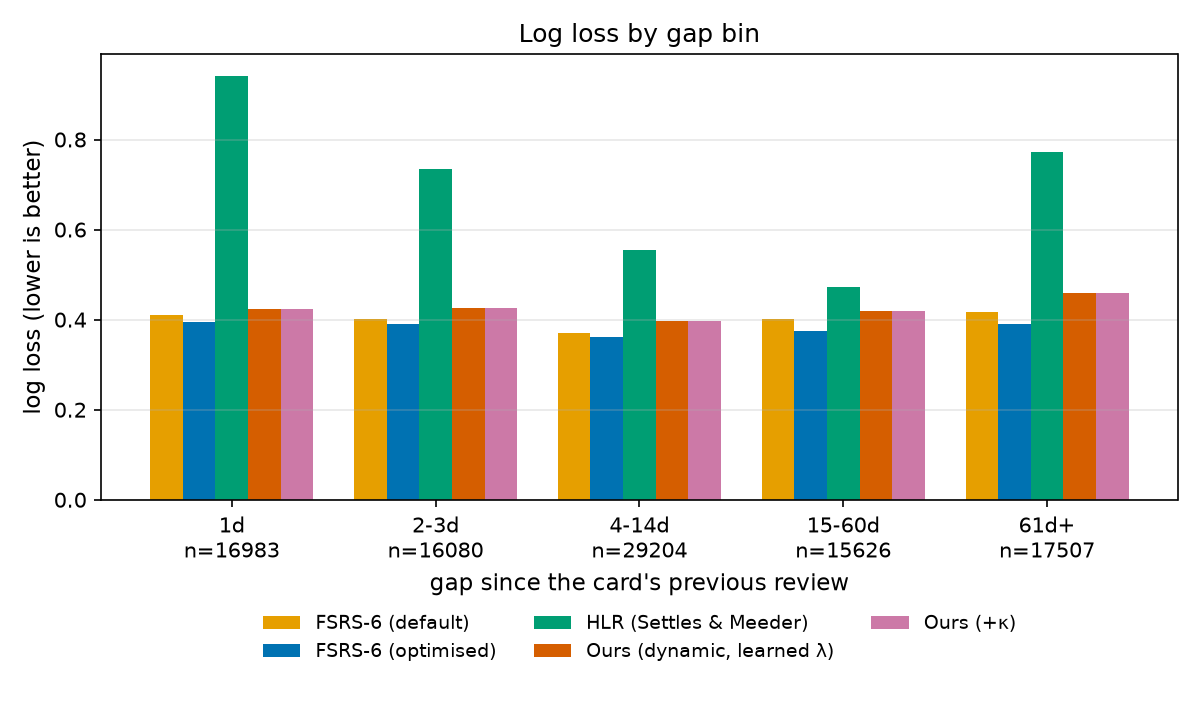
\includegraphics[width=0.82\linewidth]{../../results/full_u100_c1000/gapbins_logloss.png}
\caption{Log loss by gap bin (lower is better).}
\label{fig:gaps}
\end{figure}

The ranking is the same in every gap bin (Table~\ref{tab:gaps}, Figure~\ref{fig:gaps}): FSRS-6 (optimised), then FSRS-6 (default), then our model, then HLR. Our model's log-loss gap to FSRS-6 (optimised) is widest at long gaps (61\,d+: 0.460 against 0.389). Its AUC gap is narrowest there (0.763 against 0.817).

\subsection{Calibration}
\begin{figure}[H]
\centering
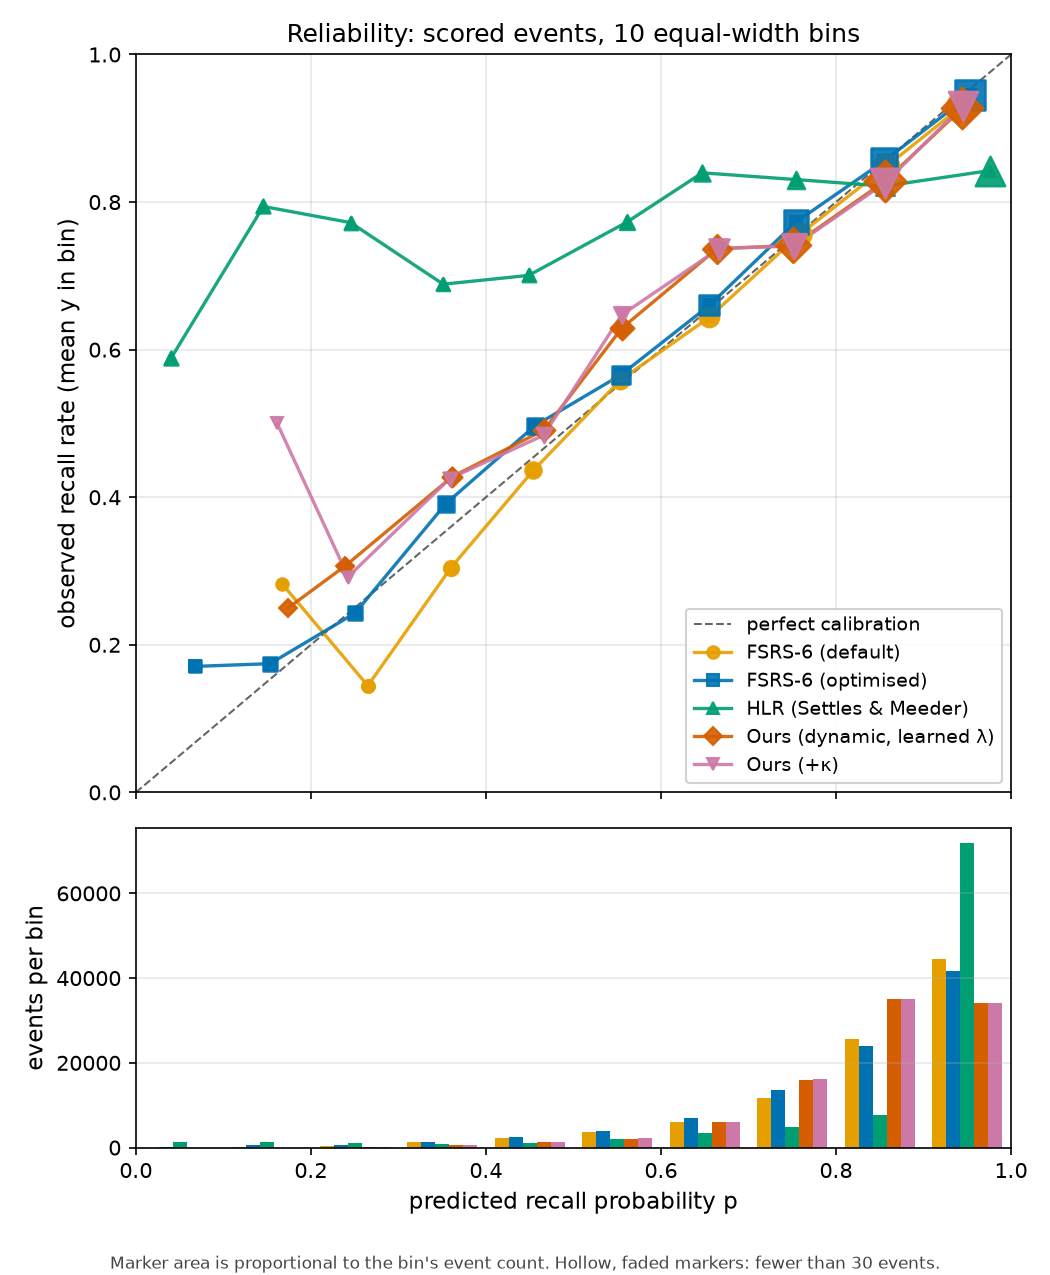
\includegraphics[width=0.66\linewidth]{../../results/full_u100_c1000/reliability.png}
\caption{Reliability diagram over all gaps (10 equal-width bins). Marker area is proportional to the bin count.}
\label{fig:rel}
\end{figure}

Both FSRS-6 variants lie close to the diagonal (Figure~\ref{fig:rel}). Our model is under-confident in the middle range: in the 0.5--0.6 bin it predicts 0.555 on average, while the observed recall is 0.629. At long gaps it becomes over-confident, with a mean bias of $+0.090$ at 61\,d+ (ECE 0.090, against 0.027 for FSRS-6 optimised). At 1\,d its bias is only $-0.006$. HLR is badly miscalibrated in both directions. Its mean bias is $+0.170$ at 1\,d and $-0.249$ at 61\,d+.

\subsection{Paired differences and per-user results}
\begin{table}[H]
\centering
\caption{Paired differences (model minus reference) with 95\% user-clustered bootstrap intervals. $^*$ marks an interval that excludes zero.}
\label{tab:paired}
\footnotesize
\setlength{\tabcolsep}{4pt}
\begin{tabular}{llll}
\toprule
Comparison & $\Delta$ Log loss & $\Delta$ Brier & $\Delta$ AUC \\
\midrule
FSRS-6 (def) $-$ FSRS-6 (opt) & $+0.017$ [0.008, 0.025]$^*$ & $+0.004$ [0.002, 0.006]$^*$ & $-0.032$ [$-$0.047, $-$0.016]$^*$ \\
Ours $-$ FSRS-6 (opt) & $+0.043$ [0.033, 0.055]$^*$ & $+0.014$ [0.011, 0.019]$^*$ & $-0.084$ [$-$0.110, $-$0.064]$^*$ \\
Ours $-$ FSRS-6 (def) & $+0.026$ [0.013, 0.042]$^*$ & $+0.011$ [0.007, 0.015]$^*$ & $-0.053$ [$-$0.087, $-$0.023]$^*$ \\
HLR $-$ Ours & $+0.258$ [0.204, 0.314]$^*$ & $+0.038$ [0.026, 0.052]$^*$ & $-0.137$ [$-$0.203, $-$0.075]$^*$ \\
Ours ($+\kappa$) $-$ Ours & $-0.000$ [$-$0.001, 0.000] & $-0.000$ [$-$0.000, 0.000] & $+0.001$ [$-$0.000, 0.002] \\
\bottomrule
\end{tabular}
\end{table}

All differences between model families are significant (Table~\ref{tab:paired}). The $\kappa$ term makes no detectable difference. Per user, FSRS-6 (optimised) has a lower log loss than our model for 78 of the 100 users, and FSRS-6 (default) for 68. Our model beats HLR for 86 users.

\subsection{MCMC convergence}
\begin{table}[H]
\centering
\caption{Posterior summaries of the poorly mixing parameters (one chain, 250 kept draws). Targets are $\hat R<1.01$ and an effective sample size (ESS) in the hundreds.}
\label{tab:mcmc}
\small
\begin{tabular}{llcccc}
\toprule
Variant & Parameter & Mean & 95\% interval & ESS & Split $\hat R$\\
\midrule
Ours & $\lambda$ & 1.871 & [1.312, 2.646] & 3.0 & 2.44 \\
Ours & $\sigma^2$ & 0.204 & [0.189, 0.231] & 3.3 & 2.07 \\
Ours & $b_0$ & 2.332 & [2.314, 2.343] & 3.9 & 1.85 \\
Ours ($+\kappa$) & $\lambda$ & 1.455 & [0.898, 2.228] & 3.0 & 2.38 \\
Ours ($+\kappa$) & $\kappa$ & $-$0.160 & [$-$0.211, $-$0.076] & 3.5 & 1.94 \\
\bottomrule
\end{tabular}
\end{table}

The chains did not converge at 2{,}000 iterations (Table~\ref{tab:mcmc}). The decay rate $\lambda$ in particular is still drifting. An attempted 8{,}000-iteration run saw $\lambda$ move from 1.52 to 1.70 between sweeps 1{,}200 and 1{,}400. That run was cut short by a machine shutdown. The other hyper-parameters mix acceptably ($\tau^2_\alpha$, $\tau^2_\gamma$ and $g_0$ have ESS of 81--250 and $\hat R \le 1.06$). The $\lambda$ Metropolis--Hastings acceptance rate is 0.24.

The predictions nevertheless appear insensitive to this. The two variants settle on clearly different $\lambda$ posteriors (means 1.87 and 1.46), yet their predictions correlate at $r=0.992$ over the 95{,}400 events, and every metric agrees to about three decimals. This suggests that the poorly mixed directions of the posterior barely move the predicted recall. It is evidence, not proof: the results for our model should be treated as provisional until a longer multi-chain run is available.

\section{Discussion}
\begin{itemize}
  \item \textbf{FSRS is the stronger model on this data.} It is better in every gap bin, on discrimination and on calibration. FSRS also models a latent memory state per card (stability and difficulty), so it is not one of the static baselines our earlier updates compared against.
  \item \textbf{Comparison with earlier claims.} Against static baselines, the continuous-time state-space approach clearly helps: our model beats HLR by 0.258 in log loss. Against FSRS, however, our model shows no long-gap advantage. At 15--60\,d and 61\,d+, FSRS-6 (optimised) has lower log loss, higher AUC and better calibration. Any claim in the group paper that the DLM fixes long-gap miscalibration should be limited to static baselines, or should report this result alongside it.
  \item \textbf{Where our model falls short.} It discriminates worse than FSRS (AUC 0.692 against 0.777), and it is over-confident at long gaps. Likely contributors are the non-converged decay rate, a single global $\lambda$ (FSRS fits its parameters per user), and the fact that our model treats a ``Hard'' answer the same as ``Good'' or ``Easy'', whereas FSRS uses all four grades.
  \item \textbf{$\kappa$.} Practice-dependent decay slowing adds nothing measurable here.
\end{itemize}

\section{Limitations}
\begin{itemize}
  \item \textbf{Convergence:} single-chain MCMC that did not converge (above). A run of 8{,}000--10{,}000 iterations with several chains and between-chain $\hat R$ is needed, at about 35~hours per 8{,}000 iterations on one CPU core.
  \item \textbf{Sample:} 100 users and at most 1{,}000 cards per user, one seed, one user sample. The bootstrap intervals reflect user sampling only, not run-to-run variation.
  \item \textbf{FSRS pipeline:} FSRS is run through \texttt{py-fsrs}, not the srs-benchmark pipeline (different split, no outlier filtering), so the numbers are not directly comparable with published leaderboards. The \texttt{py-fsrs} optimiser trains on at most the first 64 reviews of each card.
  \item \textbf{HLR:} no lexeme features, so this HLR is weaker than the original.
  \item \textbf{Scope:} same-day and first reviews are not scored. Cards with truncated histories are excluded.
\end{itemize}

\section{Reproducibility}
Code is in the \texttt{fsrs\_benchmark/} package (commit \texttt{2eaa33c}, branch \texttt{BayesianScheduler}). It has 260 tests, which run with \texttt{pytest fsrs\_benchmark/tests}. With a Hugging Face token that has accepted the dataset licence:
\begin{verbatim}
python -m fsrs_benchmark.run --run_name full_u100_c1000 --n_users 100 \
    --max_cards 1000 --seed 0 --iters 2000 --burn 1000 --workers 8
python -m fsrs_benchmark.report --run_dir results/full_u100_c1000
\end{verbatim}
FSRS and HLR take about 15 minutes. Each variant of our model takes about 7.5 hours on one core. Every run records its arguments, package versions, git commit, counts and timings in \texttt{run\_info.json}. A config fingerprint stops stale predictions from being reused. The full protocol and implementation notes are in \texttt{docs/EVALUATION.md}.

\begin{thebibliography}{9}\small
\bibitem{settles} B.~Settles and B.~Meeder. A trainable spaced repetition model for language learning. \emph{ACL}, 2016.
\bibitem{hlrcode} Duolingo. \texttt{halflife-regression} (\texttt{experiment.py}). \url{https://github.com/duolingo/halflife-regression}
\bibitem{pyfsrs} Open Spaced Repetition. \texttt{py-fsrs} 6.3.2. \url{https://github.com/open-spaced-repetition/py-fsrs}
\bibitem{data} Open Spaced Repetition. \texttt{anki-revlogs-10k}. \url{https://huggingface.co/datasets/open-spaced-repetition/anki-revlogs-10k}
\bibitem{pg} N.~G.~Polson, J.~G.~Scott and J.~Windle. Bayesian inference for logistic models using Pólya-Gamma latent variables. \emph{JASA}, 2013.
\bibitem{ck} C.~K.~Carter and R.~Kohn. On Gibbs sampling for state space models. \emph{Biometrika}, 1994.
\end{thebibliography}
\end{document}
